%
% burgerintro.tex
%
% (c) 2018 Prof Dr Andreas Müller, Hochschule Rapperswil
%
\subsection{Nichtlineare Transportgleichung\label{subsection:nichtlineare}}
Die Gleichung von Burgers in der Form
\begin{equation}
\frac{\partial u}{\partial t} + u\frac{\partial u}{\partial x}=0
\qquad\text{mit Anfangsbedingung}\qquad
u(0,x) = u_0(x)
\label{burgers:transport}
\end{equation}
modelliert ein nichtlneares Transportproblem.
Die Gleichung~\eqref{burgers:transport} ist eine quasilineare partielle
Differentialgleichung erster Ordnung, die mit der Methode der
Charakteristiken \cite{burgers:pde} gelöst werden kann.
Die Charakteristiken-Gleichungen sind
\begin{align*}
t'(s)&=1
\\ 
x'(s)&=u
\\
u'(s)&=0
\end{align*}
Aus der ersten Gleichung leitet man ab, tdass $s=t$.
Die dritte Gleichung besagt, dass $u$ entlang einer Charakteristik konstant
ist, also $u(s)=u_0$.
Die zweite Gleichung besagt dann, dass die im Punkt $(0,x_0,u_0(x_0))$
beginnende Charakteristik eine Gerade mit $x(t)=x_0 + u_0(x_0)t$ ist.

\begin{figure}
\centering
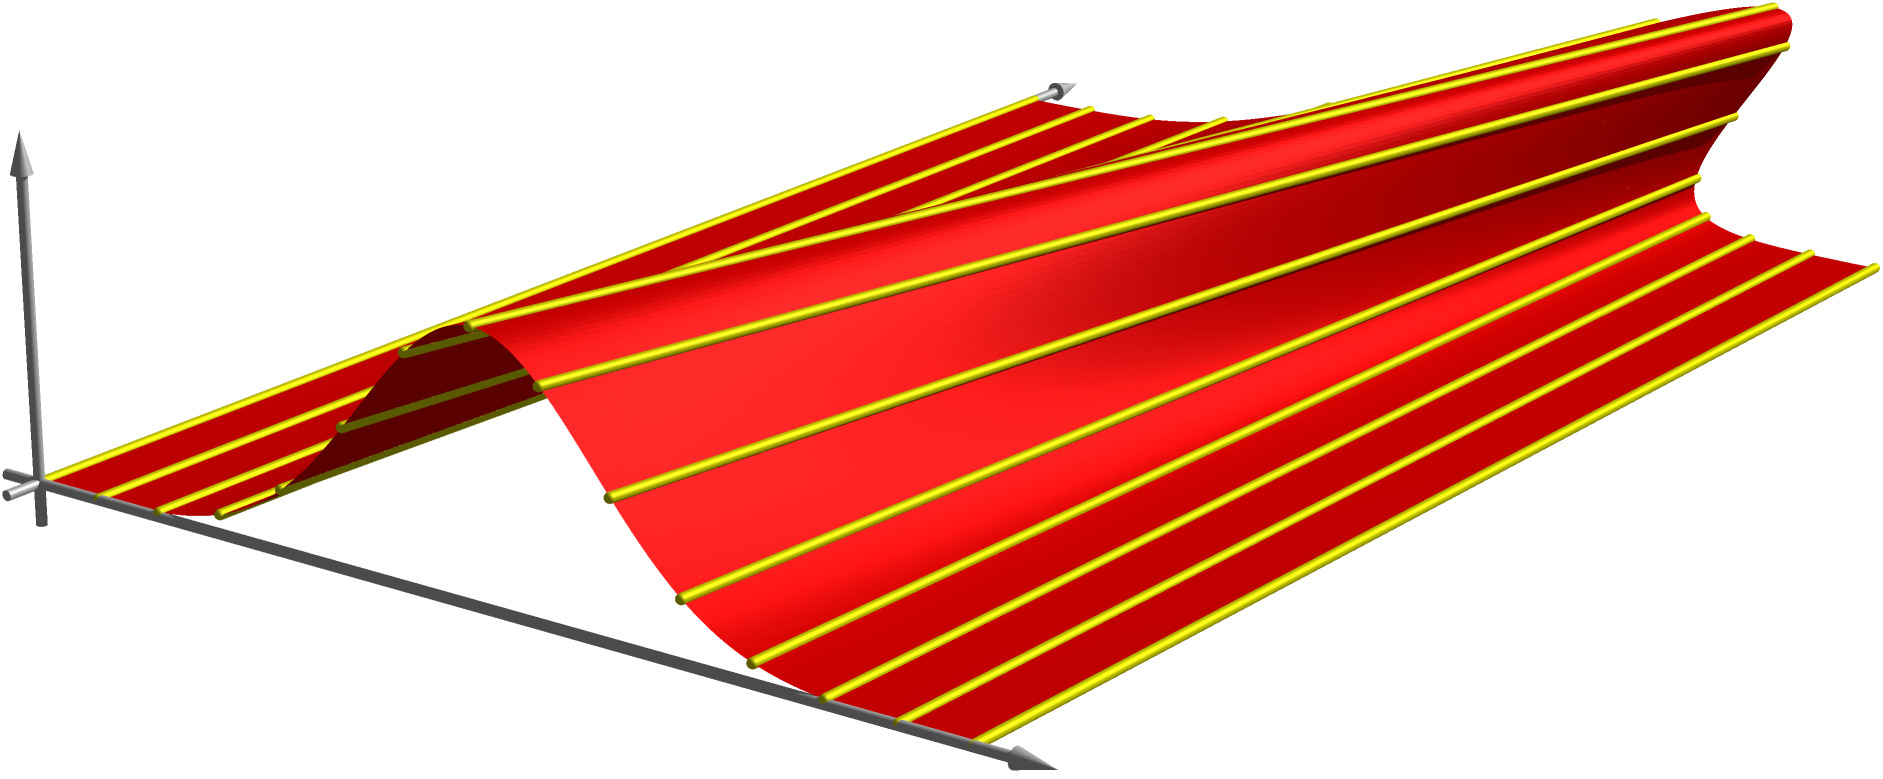
\includegraphics[width=\hsize]{learning/welle.jpg}
\caption{Lösung der Gleichung von Burgers mit Hilfe der Methode
der Charakteristiken.
Die Lösungsfläche ist darstellbar als eine Schar von Geraden (gelb).
\label{burgers:charloesung}}
\end{figure}
Die Abbildung~\ref{burgers:charloesung} 
zeigt eine Lösung mit einer Gauss-Verteilung als Anfangsbedingung.
Es ist offensichtlich, dass die gezeigte Fläche früher oder später nicht
mehr Graph einer Funktion $u(x,y)$ sein kann.
Es entwickelt sich eine Sprungstelle, die Gleichung von Burgers ist
ein Modell für eine Schockwelle.
Man kann insbesondere nicht erwarten, dass die Gleichung von Burgers
für beliebige Zeiten $t$ eine glatte Lösung hat, selbst wenn die
Anfangsbedingungen glatt waren.
Man muss sich mit einer schwachen Lösung begnügen.
Dies hat sowohl auf numerische Lösungsverfahren Auswirkungen wie auch
auf das Problem, Trainingsdaten für auf Machine Learning basierenden
Lösungsalgorithmus zu erzeugen.

\subsection{Erhaltungssatz\label{subsection:erhaltungssatz}}
Die Gleichung von Burgers kann man auch in der Form
\begin{equation}
\frac{\partial u}{\partial t}
+
\frac{\partial}{\partial x} \frac{u^2}{2}
=
0
\label{burgers:erhaltungssatz}
\end{equation}
formulieren.
Dies ist ein Spezialfall der allgemeineren Gleichung
\begin{equation}
\frac{\partial u}{\partial t}
+
\frac{\partial }{\partial x} F(u)
=
0
\label{burgers:conservationlaw}
\end{equation}
mit $F(u)=\frac12u^2$.
Man nennt 
\eqref{burgers:conservationlaw}
einen Erhaltungssatz.
Diese Betrachtungsweise erlaubt, die Bewegung von Sprungstellen besser
zu verstehen.

Die Differentialgleichung~\eqref{burgers:conservationlaw} kann auch
in der Form
\[
\frac{\partial u}{\partial t}
+
\frac{\partial }{\partial x} F(u)
=
\begin{pmatrix}
\frac{\partial}{\partial t}
\\
\frac{\partial}{\partial x}
\end{pmatrix}
\begin{pmatrix}t\\F(u)\end{pmatrix}
=
\nabla\cdot 
\begin{pmatrix}t\\F(u)\end{pmatrix}
=0
\]
schreiben.
Darauf ist aber der Satz \ref{skript:wegunabhaengigkeit} anwendbar.
Er besagt, dass Integrale
\begin{align}
\oint_\gamma(
F(u)\,dt
-
u\,dx
)
&=
\int_D \frac{\partial u}{\partial t}+\frac{\partial}{\partial x}F(u)\,dx\,dy
=
0
\label{burgers:integral}
\end{align}
über geschlossene Wege $\gamma$ verschwinden.

\subsection{Hugoniot-Rankine-Bedingungen\label{subsection:hugnoniot}}
\begin{figure}
\centering
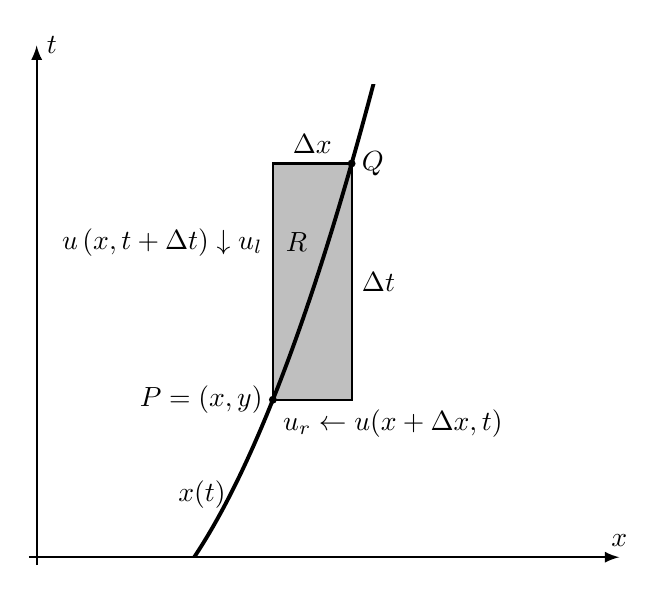
\begin{tikzpicture}[>=latex,thick]
\fill[color=gray!50] (3,2)--(4,2)--(4,5)--(3,5)--cycle;
\node at (3.3,4.0) {$R$};
\draw[->] (-0.1,0)--(7.4,0) coordinate[label={$x$}];
\draw[->] (0,-0.1)--(0,6.5) coordinate[label={right:$t$}];
\fill (3,2) circle[radius=0.05];
\node at (3,2) [left] {$P=(x,y)$};
\fill (4,5) circle[radius=0.05];
\node at (4,5) [right] {$Q$};
\draw (3,2)--(4,2)--(4,5)--(3,5)--cycle;
\node at (3.5,5) [above] {$\Delta x$};
\node at (4,3.5) [right] {$\Delta t$};
\begin{scope}
\clip (0,0) rectangle (7,6.0);
\draw[line width=1.4pt] plot[domain=2:5,samples=100] ({\x},{0.5*\x*\x -0.5*(\x)-1});
\end{scope}
\node at (3,4) [left] {$\begin{matrix}u(x,t+\Delta t)\\\downarrow\\u_l\end{matrix}$};
\node at (3,2) [below right] {$u_r\leftarrow u(x+\Delta x,t)$};
\node at (2.1,0.8) {$x(t)$};
\end{tikzpicture}
\caption{Herleitung der Hugoniot-Rankine-Bedingung für die Bewegung einer
Sprungstelle der Lösung eines Erhaltungssatzes.
\label{burgers:hugoniot}}
\end{figure}
In Abschnitt~\ref{subsection:nichtlineare} haben wir gesehen, dass Lösungen
der Gleichung von Burgers Sprungstellen entwickeln.
Die Formulierung als Erhaltungssatz in
Abschnitt~\ref{subsection:erhaltungssatz} 
soll uns jetzt erlauben, die Bewegung solcher Sprungstellen zu beschreiben.

Sie also $u(t,x)$ eine Lösung fast überall der Gleichung von Burgers mit
einer Sprungstelle, die sich entlangt der Kurve $x(t)$ bewegt.
Dazu berechnen wir das Wegintegral \eqref{burgers:integral} über den Rand
des Rechtecks mit den Ecken $(x,y)$ und $(x+\Delta x, y+\Delta y)$.
Wir benötigen die Grenzwerte
\[
\begin{aligned}
u_l &= \lim_{\Delta t\to 0+} u(t+\Delta t,x)
&&\text{und}&
u_r &= \lim_{\Delta x\to 0+} u(t,x+\Delta x).
\end{aligned}
\]
Damit können wir das Wegintegral approximieren als
\begin{align}
\int_{\partial R}(u\,dx -F(u)\,dt)
&=
0
\notag
\\
u(t+\Delta t,x)
\Delta x
-
F(u(t+\Delta t,x))
\Delta t
&=
u(t,x+\Delta x) \Delta x
-
F(u(t,x+\Delta x)) \Delta t
\notag
\\
\Delta x
(
u(t+\Delta t,x)
-
u(t,x+\Delta x)
)
&=
\Delta t
(F(u(t+\Delta t,x))
-
F(u(t,x+\Delta x))
)
\notag
\\
\intertext{Oder nach Grenzübergang $\Delta t\to 0$ und $\Delta x\to 0$}
\dot x(t)\, (u_l-u_r) &= F(u_l) - F(u_r).
\label{burgers:hugoniot-rankine}
\end{align}
Die Geschwindigkeit, mit der sich die Sprungstelle bewegt, hängt also 
von den Werten von $u(t,x)$ auf beiden Seiten der Sprungstelle ab.
Dies sind die {\em Hugoniot-Rankine-Bedingungen}.
Wir werden sie Abschnitt~\ref{burgers:training} verwenden, um Trainingsdaten
für Sprungstellen der Lösung zu erzeugen.
\index{Hugoniot-Rankine-Bedingungen}
\index{Rankine-Hugoniot-Bedingungen}


\subsection{Numerische Lösungen und Computational mode}
Bei der numerischen Lösung der Gleichung von Burgers tritt erschwehrend der
Computational Mode auf.

